\begin{figure}[h]
      \centering   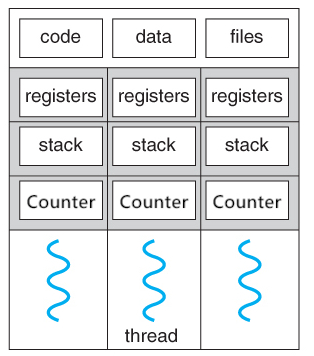
\includegraphics[scale=2]{./images/threads_01.jpeg}
\end{figure}

\begin{enumerate}
    \item
    \item
\end{enumerate}

\begin{myTableStyle}
    \begin{tabular}{ |m{8cm}|m{8cm}| } \hline
        User thread             &     Kernel Thread         \\ \hline
        Implemented by user     &     Implemented by OS.    \\ \hline
    \end{tabular}
\end{myTableStyle}
\vspace{0.08in}

\fillin[]



                TLB access time                     &   \(t_b\)         \\ \hline
                main memory access time             &   \(t_m\)         \\ \hline
                TLB access time                     &   \(t_b\)         \\ \hline
                TLB access time                     &   \(t_b\)         \\ \hline



